\documentclass{article}

\usepackage{graphicx}
\usepackage{multicol}
\usepackage[latin1]{inputenc} % package caracteres francais
\usepackage[T1]{fontenc}      % package caracteres francai
\usepackage[francais]{babel}  % package caracteres francai
\usepackage{vmargin}
\setmarginsrb{20mm}{20mm}{20mm}{20mm}{0mm}{0mm}{4mm}{8mm}

\begin{document}


%======Page de garde=======
\begin{center}

\includegraphics[width=10cm]{logoULFST.jpg} %l'image est retaill\'ee pour avoir une largeur de 10cm
\end{center}

\begin{center}
\thispagestyle{empty}
{\bfseries \large Master Informatique}
\end{center}

\vspace*{70mm}
\begin{center}
	{\bfseries \Huge Rapport du projet d'initiation \`{a} la recherche}
\end{center}
\vspace*{10mm}
\begin{center}
{\large sujet : Constitution d'une base de cas de corrections du fran\c{c}ais}
\end{center}
\begin{center}
{\large Ann\'ee 2018-2019}
\end{center}



\vspace*{60mm}
\begin{multicols}{2}
\begin{multicols}{2}
	\begin{flushright}
		\`{E}tudiants :
	\end{flushright}
		\vfill\null\columnbreak
	\begin{flushleft}
		Alex Ginestra\newline Christopher Klein
	\end{flushleft}
\end{multicols}
\vfill\null\columnbreak
\begin{multicols}{2}
	\begin{flushright}
		\`{E}quipe :
	\end{flushright}
	\begin{flushright}
		Encadrants :
	\end{flushright}
	\vfill\null\columnbreak
	\begin{flushleft}
	Orpailleur et S\'emagramme\newline Bruno Guillaume, Yves Lepage, Jean Lieber et Emmanuel Nauer
	\end{flushleft}
\end{multicols}
\end{multicols}
\cleardoublepage
\cleardoublepage


%=====Decharge de responsabilite=====
\thispagestyle{empty}
\begin{center}
{\bfseries \huge D\'echarge de responsabilit\'e}
\end{center}
\vspace*{10mm}

L'Universit\'{e} de Lorraine n'entend donner ni approbation ni improbation aux opinions \'{e}mises dans ce rapport, ces opinions devant \^{e}tre consid\'{e}r\'{e}es comme propres \`{a} leur auteur.
\cleardoublepage


%=====Page remerciements=====
\thispagestyle{empty}
\begin{center}
{\bfseries \huge Remerciements}
\end{center}
\vspace*{10mm}

Tout d'abord, nous tenons \`{a} remercier toute l'\'{e}quipe p\'{e}dagogique du d\'{e}partement informatique de la facult\'{e} des sciences et technologies pour les quatre ann\'{e}es de formation en Master informatique.
De plus, nous remercions toutes les personnes qui ont contribu\'{e} au bon d\'{e}roulement de notre travail et qui nous ont aid\'{e} lors de la r\'{e}daction de ce rapport. Premi\`{e}rement, nous adressons nos remerciements \`{a} notre professeur, Madame Marie-Laure Alves, qui nous a beaucoup aid\'{e}. Son \'{e}coute et ses conseils nous ont permis de progresser dans notre d\'{e}marche.
Nous tenons \'{e}galement \`{a} remercier vivement notre encadrant, Monsieur Jean Lieber, enseignant chercheur au LORIA, pour son accueil, le temps pass\'{e} ensemble et le partage de son expertise au quotidien. Nous remercions \'{e}galement toute l'\'{e}quipe K et l'\'{e}quipe S\'{e}magramme pour leur accueil et leur disponibilit\'{e}, et en particulier Monsieur Emmanuel Nauer, qui nous a beaucoup aid\'{e} \`{a} comprendre les probl\'{e}matiques de recherche sur lesquelles nous travaillions. Enfin, nous tenons \`{a} remercier toutes les personnes qui nous ont conseill\'{e} et relu lors de la r\'{e}daction de ce rapport : nos familles, nos professeurs et aussi nos camarades de cours.

\cleardoublepage


%======Sommaire====== 
\begin{center}
{\bfseries \huge Sommaire}
\end{center}
\tableofcontents


\setcounter{page}{3}

\cleardoublepage

%=====Rappel du sujet====
\begin{center}
{\bfseries \huge Rappel du sujet}
\end{center}

\vspace*{10mm}


{\bfseries Probl\'ematique de recherche : }
\newline
\vspace*{2mm}

Le raisonnement \`{a} partir de cas (R\`{a}PC) est un raisonnement hypoth\'etique (en g\'en\'eral) qui consiste \`{a} r\'esoudre un nouveau probl\`{e}me (le probl\`{e}me cible, not\'e cible) en s'appuyant sur une base de cas, un cas \'etant la repr\'esentation d'un \'episode de r\'esolution de probl\`{e}me. On appelle cas source un \'el\'ement de la base de cas. Souvent, on repr\'esente un cas source simplement par un couple (srce, sol(srce)) : srce est un probl\`{e}me source, sol(srce) est une solution de ce probl\`{e}me source. Un mod\`{e}le du processus de R\`{a}PC classique comprend deux \'etapes d'inf\'erence : 
Rem\'emoration : un cas source (srce, sol(srce)) jug\'e similaire au probl\`{e}me cible (par exemple, sur la base d'une distance entre probl\`{e}mes) est s\'electionn\'e. 
Adaptation : La solution sol(srce) de ce cas est modifi\'ee en une solution candidate sol(cible) de cible. 

La correction de phrases est la probl\'ematique de la transformation d'une phrase incorrecte (en particulier, grammaticalement) en une phrase corrig\'ee (nous choisirons la langue fran\c{c}aise dans ce travail, m\^eme si la probl\'ematique existe dans toutes les langues). Un cas de correction de phrase est donc un couple (srce, sol(srce)) o\`{u} srce est une phrase incorrecte et sol(srce) une correction de srce. Par exemple, on a les deux cas : 
srce1 = Tu as pas mang\'e. sol(srce1) = Tu n'as pas mang\'e. 
srce2 = Il a recommencer. sol(srce2) = Il a recommenc\'e. 
L'adaptation se fait par des techniques de raisonnement par analogie : la solution sol(cible) est solution d'une \'equation analogique << srce est \`{a} sol(srce) ce que cible est \`{a} y >>. Par exemple, l'adaptation de (srce2, sol(srce2)) \`{a} cible = Tu as manger. consiste \`{a} r\'esoudre Il a recommencer. est \`{a} Il a recommenc\'e. ce que Tu as manger. est \`{a} x qui a pour solution, avec la relation d'analogie utilis\'ee dans le projet, x = Tu as mang\'e., proposition de solution propos\'ee par le syst\`{e}me. 
Sujet : 
Comme pour tout syst\`{e}me \`{a} base de connaissances, la qualit\'e d'un syst\`{e}me de R\`{a}PC d\'epend de celle de son moteur d'inf\'erences mais \'egalement de la qualit\'e de sa base de connaissances, en particulier de sa base de cas. Une bonne base de cas doit avoir plusieurs qualit\'es. Les cas sources doivent \^etre corrects. Elle doit avoir une bonne couverture (et permettre de r\'esoudre correctement une proportion importante de cas). Elle devrait ne pas \^etre trop redondante (certains cas diff\'erents correspondent \`{a} la m\^eme correction). 
Pour cela, on pourra consulter les mouchards d'\'edition de Wikip\'edia pour en extraire des listes de fautes grammaticales ou orthographiques typiques, ainsi que des sites de dict\'ees ou d'orthographe. Il faudra mettre en place les outils de collecte automatiques, param\'etrables en fonction des sites. 
Une autre piste est la mise en place d'un jeu interactif avec un but. Le but est de faire corriger des phrases fautives par les joueurs. La phrase corrig\'ee devrait \'emerger de la majorit\'e des propositions de correction. Les phrases fautives pourraient \^etre extraites de listes d'exemples fautifs, ou produites automatiquement \`{a} partir de patrons pr\'ed\'efinis ou par application de l'analogie sur des cas d\'ej\`{a} collect\'es.
Une courte \'etude bibliographique sur la maintenance de base de cas permettra de sugg\'erer des pistes pour l'acquisition d'une bonne base de cas. Il faudra mettre en place une m\'ethode pour cela, qui pourra s'appuyer sur les sites mentionn\'es ci-dessus.

\cleardoublepage


%===== Introduction ====
\begin{center}
{\bfseries \huge Introduction}
\end{center}

\vspace*{35mm}


Le TAL (traitement automatique des langues) est un domaine d'\'{e}tude dont l'objectif est de cr\'{e}er des outils de traitement de la langue pour diverses applications. Il traite de nombreux sujets notamment dans le domaine de la compr\'{e}hension automatique des textes, la traduction automatique, ou encore la correction automatique des fautes orthographiques et grammaticales. C'est pourquoi linguistes et informaticiens collaborent \'{e}troitement sur l'\'{e}tude de la langue et le traitement automatique des donn\'{e}es. Le traitement automatique du langage couvre donc un large panel de disciplines de recherche et se trouve \`{a} l'origine de nombreux travaux. 
\newline
Parmi les premiers travaux, qui remontent aux ann\'{e}es 50 pendant la guerre froide, se trouve la mise au point du premier traducteur automatique. Nomm\'{e} "experience Georgetown-IBM" et d\'{e}velopp\'{e} par l'universit\'{e} de Georgetown en collaboration avec la soci\'{e}t\'{e} IBM, le projet offrait la possibilit\'{e} de traduire du russe vers l'anglais. C'est en 1954 que la premi\`{e}re d\'{e}monstration sur une soixantaine de phrases s'est faite, une vraie prouesse technologique pour l'\'{e}poque. Depuis, le traitement automatique des langues a bien \'{e}volu\'{e} et est devenu un domaine pluridisciplinaire. Il peut allier la linguistique, l'informatique, et m\^{e}me se coupler \`{a} de l'intelligence artificielle pour cr\'{e}er des applications de plus en plus complexes nous permettant de simplifier nos t\^{a}ches quotidiennes. 
\newline

Un correcteur automatique de la langue est un exemple d'outil utilisant des domaines du traitement automatique des langues. Il utilise des disciplines de recherche vari\'{e}es telles que l'analyse syntaxique, la correction orthographique et d'autres plus sp\'{e}cifiques telles que la d\'{e}limitation de phrase ou la morphologie. Un outil tel que celui-ci est un monstre de conception et de d\'{e}veloppement, et les meilleurs correcteurs automatiques connus \`{a} ce jour ont \'{e}t\'{e} d\'{e}velopp\'{e}s par des entreprises internationales comme Microsoft, Google ou encore Apple. 
\newline

Contrairement aux cas d\'{e}crits pr\'{e}c\'{e}demment, notre sujet consiste \`{a} cr\'{e}er un syst\`{e}me permettant la correction automatique de phrases fran\c{c}aises en s'appuyant sur le raisonnement \`{a} partir de cas (R\`{a}PC). Pour r\'{e}pondre \`{a} cette probl\'{e}matique, nous allons tout d'abord introduire le raisonnement \`{a} partir de cas et expliquer comment il va nous permettre de corriger des phrases. Puis nous aborderons une partie plus pratique o\`{u} nous d\'{e}taillerons les diff\'{e}rentes \'{e}tapes permettant de r\'{e}soudre notre probl\'{e}matique. Nous parlerons ensuite des r\'{e}sultats obtenus suite \`{a} nos d\'{e}veloppements et finirons par introduire les suites possibles de notre projet.
\newline

\cleardoublepage


%===== 1ere partie ====
\section{Analyse du probl\`{e}me et organisation}

%===== 1ere sous partie ====
\subsection{Le raisonnement \`{a} partir de cas}
Le raisonnement \`{a} partir de cas (not\'{e} R\`{a}PC) est un raisonnement qui consiste \`{a} r\'{e}soudre des probl\`{e}mes de la vie quotidienne s'appuyant sur des exp\'{e}riences similaires rencontr\'{e}es par le pass\'{e}. Gr\^{a}ce aux exp\'{e}riences pass\'{e}es d\'{e}j\`{a} r\'{e}solues, nous arrivons \`{a} en inf\'{e}rer une solution qui s'ajoute \`{a} notre exp\'{e}rience. La reproduction de cet exemple un grand nombre de fois nous permettra d'avoir une exp\'{e}rience telle que nous pouvons essayer de d\'{e}duire une solution \`{a} n'importe quel probl\`{e}me ressemblant.
\newline
\newline
Il y a deux principales \'{e}tapes dans ce raisonnement. Premi\`{e}rement, il y a ce qu'on appellera la "rem\'{e}moration", qui est le rapprochement entre notre probl\`{e}me actuel (que nous appellerons probl\`{e}me cible) et un probl\`{e}me qui a d\'{e}j\`{a} \'{e}t\'{e} r\'{e}solu dans le pass\'{e} (qu'on nommera probl\`{e}me source). La seconde \'{e}tape s'appelle "l'adaptation". Ce principe permet d'obtenir une solution de notre probl\`{e}me source en modifiant la solution du probl\`{e}me cible.
\newline
\newline
%==== image ====
\begin{center}
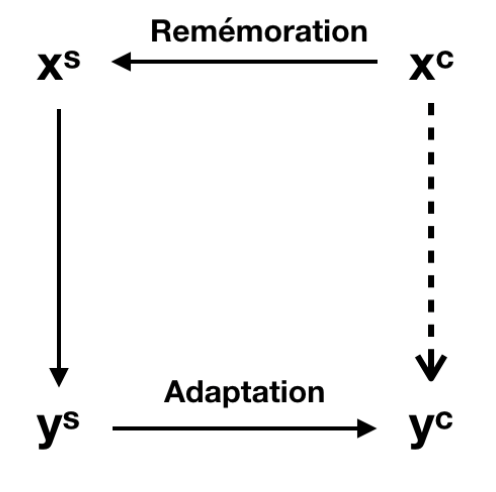
\includegraphics[width=7cm]{img1.png} %l'image est retaill\'ee pour avoir une largeur de 10cm
\end{center}

Nous voyons donc qu'il est possible de r\'{e}soudre des probl\`{e}mes gr\^ace au raisonnement \`{a} partir de cas. N\'{e}anmoins, pour pouvoir les r\'{e}soudre, nous devons avoir des probl\`{e}mes similaire d\'{e}j\`{a} r\'{e}solus. Cet ensemble de couples (probl\`{e}me, solution) r\'{e}solu s'appelle une base de cas. En plus du couple (probl\`{e}me, solution), une explication est ajout\'{e}e et permet d'am\'{e}liorer l'\'{e}tape de la rem\'{e}moration.
\newline
\newline
Voici un exemple de r\'{e}solution de probl\`{e}me gr\^ace au raisonnement \`{a} partir de cas : 
Voici le probl\`{e}me que nous rencontrons (probl\`{e}me cible) : <<Tu n'as pas manger>>.
Nous avons dans notre base de cas un couple tel que celui-ci : <<Il a recommencer>> est le probl\`{e}me source et <<Il a recommenc\'{e}>> est la solution du probl\`{e}me source.
La rem\'{e}moration va donc rapprocher notre probl\`{e}me cible du probl\`{e}me source et en utilisant la solution du probl\`{e}me source ainsi que l'explication, l'Adaptation va pouvoir nous fournir une solution de notre probl\`{e}me cible qui sera <<Tu n'as pas mang\'{e}>>.
\newline
\newline
Pour parvenir \`{a} r\'{e}soudre notre probl\'{e}matique qui est la correction automatique du fran\c{c}ais \`{a} l'aide du raisonnement \`{a} partir du cas, il nous faut donc une base de cas qui permette en th\'{e}orie de corriger toutes les erreurs possible du fran\c{c}ais. En prenant en compte tous les types d'erreurs possibles (grammaire, orthographe, conjugaison, etc.), il y aurait un nombre immense de cas \`{a} d\'{e}finir dans notre base, ce qui est impossible \`{a} construire \`{a} la main. Le but de notre projet est donc de construire une base de cas \`{a} l'aide d'outils diverses et vari\'{e}s qui serait totalement automatis\'{e}e.
\newline
\newline
Nous voyons donc qu'il est possible de r\'{e}soudre des probl\`{e}mes gr\^{a}ce au raisonnement \`{a} partir de cas. Cependant, pour pouvoir les r\'{e}soudre, il est n\'{e}cessaire d'avoir des probl\`{e}mes similaires d\'{e}j\`{a} r\'{e}solus. Cet ensemble de couples (probl\`{e}me, solution) r\'{e}solus s'appelle une base de cas. En plus du couple (probl\`{e}me, solution), une explication est ajout\'{e}e et permet d'am\'{e}liorer l'\'{e}tape de la rem\'{e}moration.
\newline
\newline
Voici un exemple de r\'{e}solution de probl\`{e}me gr\^{a}ce au raisonnement \`{a} partir de cas : 
Voici le probl\`{e}me que nous rencontrons (probl\`{e}me cible) : "Tu n'as pas manger".
Nous avons dans notre base de cas un couple tel que celui-ci : "Il a recommencer" est le probl\`{e}me source et "Il a recommenc\'{e}" est la solution du probl\`{e}me source.
La rem\'{e}moration va donc rapprocher notre probl\`{e}me cible du probl\`{e}me source. Puis en utilisant la solution du probl\`{e}me source ainsi que l'explication, l'adaptation va pouvoir nous fournir une solution de notre probl\`{e}me cible qui sera "Tu n'as pas mang\'{e}".
\newline
\newline
Pour parvenir \`{a} r\'{e}soudre notre probl\'{e}matique qui est la correction automatique du fran\c{c}ais \`{a} l'aide du raisonnement \`{a} partir du cas, il nous faut donc une base de cas qui permette en th\'{e}orie de corriger toutes les erreurs possibles du fran\c{c}ais. En prenant en compte tous les types d'erreurs possibles (grammaire, orthographe, conjugaison, etc.), il y aurait un nombre immense de cas \`{a} d\'{e}finir dans notre base, ce qui s'av\'{e}rerait long et fastidieux \`{a} construire \`{a} la main. Le but de notre projet est donc de construire une base de cas \`{a} l'aide d'outils qui permettrait une certaine automatisation du remplissage. 


%===== 2eme sous partie ====
\subsection{Travail existant}

Une premi\`{e}re piste nous a \'{e}t\'{e} fournie par un groupe d'\'{e}tudiants de L3 de 2017-2018 compos\'{e} de M. Giang, M. Levy, M. Ly, qui avaient travaill\'{e} sur un projet intitul\'{e} Corrector. Le projet consistait \`{a} faire un site Internet capable d'apporter une correction \`{a} une phrase erron\'{e}e donn\'{e}e en entr\'{e}e. Cette correction devait se faire \`{a} l'aide d'une base de cas qui pouvait s'enrichir avec des interactions humaines (utilisateur/administrateur du site). 
\newline
\newline
Notre d\'{e}but d'\'{e}tude a donc \'{e}t\'{e} guid\'{e} par les moyens mis en oeuvre pour effectuer un remplissage automatique de leur base de cas initiale, et plus particuli\`{e}rement un : les corpus de WiCoPaCo (Wikipedia Correction and Paraphrase Corpus). Le site WiCoPaCo met en libre acc\`{e}s des fichiers au format XML contenant des phrases, ou parties de phrases avec une correction effectu\'{e}e ainsi qu'un commentaire \'{e}ventuel laiss\'{e} par l'auteur de la correction. Ces fichiers sont le r\'{e}sultat des corrections faites par les administrateurs des pages Wikip\'{e}dia, ce qui n\'{e}cessite une correction \'{e}tant donn\'{e} que le contenu des pages est apport\'{e} par des utilisateurs. Les fichiers en question contiennent donc des centaines de milliers de cas compos\'{e}s de la mani\`{e}re suivante : le groupe de phrase avant modification avec la mise en \'{e}vidence de la faute, suivi du m\^{e}me groupe de phrase avec la correction apport\'{e}e \'{e}galement mise en \'{e}vidence. 
\newline
\newline
L'int\'{e}r\^{e}t principal de ces fichiers \'{e}tant l'\'{e}norme masse de donn\'{e}es qu'ils contiennent, nous permettant ainsi d'en extraire un grand nombre de cas. Cependant, m\^{e}me si cette solution semble \^{e}tre id\'{e}ale et simple \`{a} mettre en place, il s'av\`{e}re qu'elle est loin d'\^{e}tre parfaite. Car sur ces corrections, une partie \'{e}tant des corrections de contenu, une autre \'{e}tant des reformulations, et bien d'autres types de corrections n'\'{e}tant pas des erreurs de fran\c{c}ais mais sont pourtant contenues dans ces fichiers. La probl\'{e}matique de l'\'{e}puration de cette \'{e}norme masse de donn\'{e}es se pose donc.
\newline
\newline
Face \`{a} ce probl\`{e}me, le groupe d'\'{e}tudiants de L3 avait mis en place un script python qui prenait un fichier XML en entr\'{e}e et produisait en fichier CSV en sortie. Le script s'occupait aussi de la suppression de certains cas : les retours en arri\`{e}re. Il ne retenait donc pas les cas qui \'{e}taient des retours sur correction, c'est \`{a} dire lorsque le correcteur transformait une phrase A en phrase B, puis transformait \`{a} nouveau la phrase B en phrase A.
\newline
\newline
C'est donc en reprenant cette base de travail que nous avons d\'{e}but\'{e} notre projet, dans l'optique de pouvoir \'{e}purer cette \'{e}norme masse de donn\'{e}es \`{a} l'aide de filtres pour obtenir uniquement des cas de corrections de langue.




%===== 3eme sous partie ====
\subsection{Mise en place du projet}
Pour mettre en place notre projet, nous avons donc grandement utilis\'{e} le travail d\'{e}j\`{a} effectu\'{e} par nos coll\`{e}gues qui nous ont pr\'{e}c\'{e}d\'{e}s. Nous avons d\'{e}cid\'{e} d'utiliser l'\'{e}norme quantit\'{e} de cas que nous fournissait les fichiers XML de WiCoPaCo pour cr\'{e}er notre base de cas automatiques. Ces fichiers regroupant plus de 200 000 cas, elle serait suffisamment cons\'{e}quente pour couvrir un maximum d'erreur de fran\c{c}ais. N\'{e}anmoins, comme cela a \'{e}t\'{e} expliqu\'{e} ci-dessus, nous ne pouvons pas seulement transformer ces fichiers directement en une base de cas car un grand nombre de cas n'est pas exploitable. Nous devons donc reprendre le travail qui a \'{e}t\'{e} fait en amont et continuer \`{a} filtrer les cas jusqu'\`{a} obtenir un ensemble de cas corrects.
\newline
\newline
\`{a} la suite d'une r\'{e}flexion sur le d\'{e}veloppement de notre projet, nous avons d\'{e}cid\'{e} de ne pas reprendre les travaux effectu\'{e}s par les \'{e}tudiants pr\'{e}c\'{e}dent pour plusieurs raisons : premi\`{e}rement, bien que nous comprenions l'id\'{e}e directrice du d\'{e}veloppement, nous n'avions pas toutes les subtilit\'{e}s pour comprendre parfaitement le code. De plus, nous avions dans l'optique d'impl\'{e}menter plusieurs filtres afin de rendre la cr\'{e}ation de ceux-ci plus facile. Nous nous sommes donc r\'{e}solus \`{a} utiliser le langage orient\'{e} objet Java pour le d\'{e}veloppement de notre application. C'est un langage que nous avons eu l'habitude d'utiliser au cours de nos \'{e}tudes. Il permet de lire et d'\'{e}crire des fichiers ais\'{e}ment et permet, une fois le projet structur\'{e}, une impl\'{e}mentation simple et rapide de nouvelles fonctionnalit\'{e}s.
\newline
\newline
Cependant, notre projet consistant \`{a} trouver la correction d'une phrase de fran\c{c}ais en utilisant une base de cas, nous n'avons par cons\'{e}quent pas acc\`{e}s \`{a} un analyseur syntaxique ou orthographique pour pouvoir d\'{e}tecter si une phrase contient des erreurs. Nos encadrants nous ont demand\'{e} de r\'{e}fl\'{e}chir \`{a} une m\'{e}thode permettant d'accomplir cette d\'{e}tection.


%===== 2eme partie ====
\section{Conception et d\'{e}veloppement}

%===== 1ere sous partie ====
\subsection{D\'{e}but du d\'{e}veloppement}
Suite \`{a} la mise en place de notre sujet, nous nous sommes donc concentr\'{e}s sur deux axes principaux : la d\'{e}couverte d'un outil permettant la d\'{e}tection d'erreurs dans une phrase et le d\'{e}but du d\'{e}veloppement de notre projet en Java.

%===== 1ere sous sous partie ====
\subsubsection{Grew}
Le premier de nos deux axes \'{e}tait la d\'{e}couverte d'un outil permettant l'analyse des phrases pour en trouver les potentielles fautes de fran\c{c}ais. Pour cela, nos encadrants nous ont orient\'{e}s vers GREW, un logiciel dont un de nos encadrants, Bruno Guillaume, conna\^{i}t bien le fonctionnement. Ce logiciel permet, \`{a} partir d'une ou plusieurs phrases donn\'{e}es en param\`{e}tres, de construire un graphe \`{a} partir des lemmes de chaque mot ainsi que gr\^{a}ce au contexte des phrases. Ce graphe permet de d\'{e}duire les liens que chaque mot entretient avec les autres mots de la phrase. Voici un exemple de graphe que cr\'{e}e l'outil GREW \`{a} partir de la phrase "C'est une femme tr\`{e}s intelligente."

%==== image ====
\begin{center}
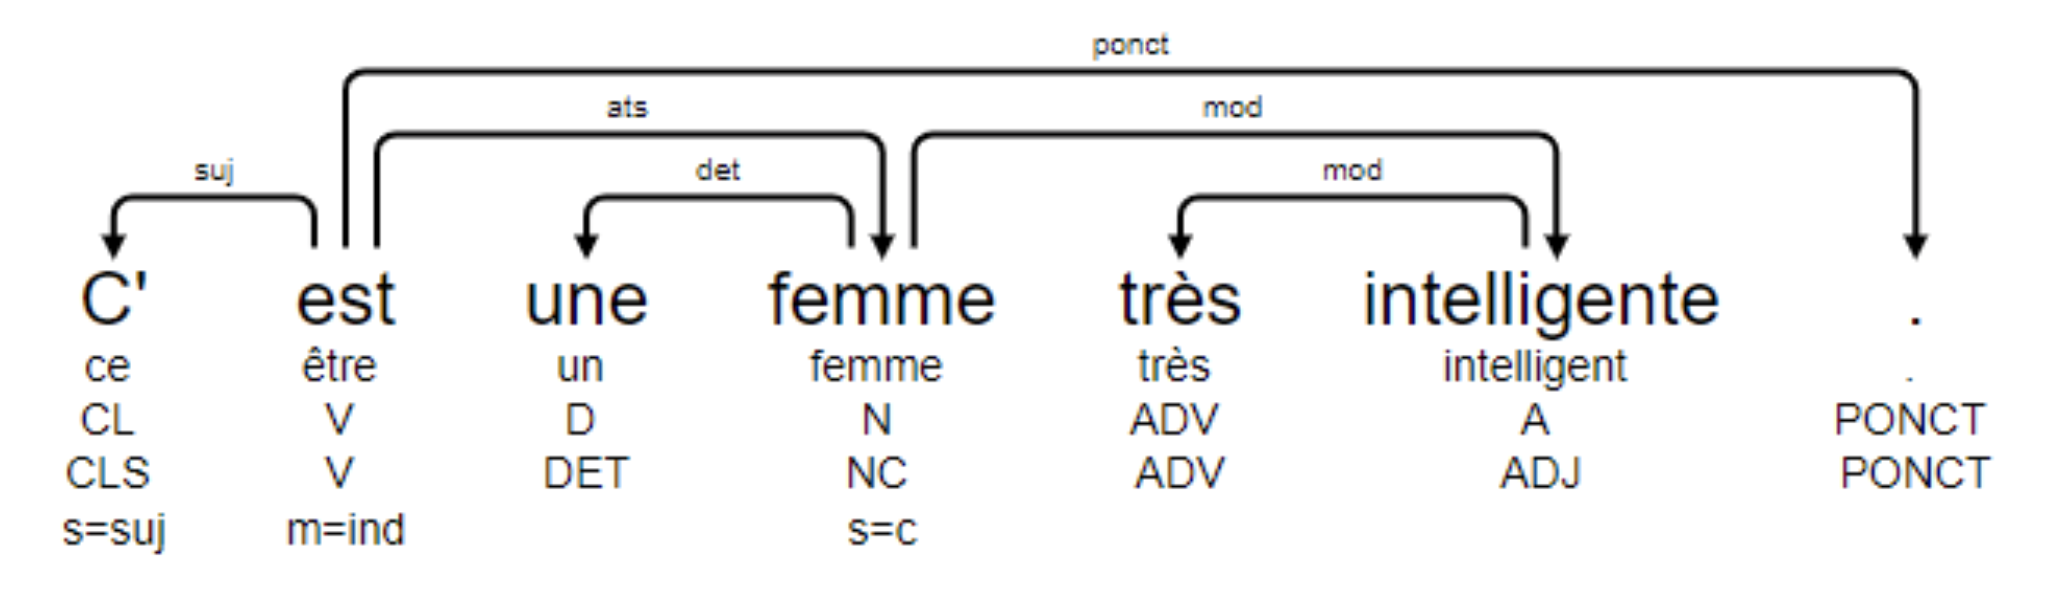
\includegraphics[width=10cm]{graphgrew.png} %l'image est retaill\'ee pour avoir une largeur de 10cm
\end{center}

Nous pouvons donc retrouver dans ce graphe le lemme de chaque mot, situ\'{e} sous le mot correspondant ainsi que les liens qu'il a avec les autres, repr\'{e}sent\'{e}s par des fl\`{e}ches qui lie les mots entre eux. Cet outil n'est donc pas un outil de d\'{e}tection d'erreur \`{a} proprement parl\'{e}. Cependant il permet, si une phrase n'est pas bien assembl\'{e} ou dans les cas o\`{u} il n'arrive pas \`{a} trouver les liens entre les mots d'une phrase, de cr\'{e}er des graphes o\`{u} tous les mots ne sont pas li\'{e}s entre eux. Prenons par exemple la phrase utilis\'{e}e dans le graphe pr\'{e}c\'{e}dent et remplaçons Le "C'est" par "S'est", ce qui est une erreur classique de français. Dans ce cas, GREW r\'{e}alise le graphe suivant :

%==== image ====
\begin{center}
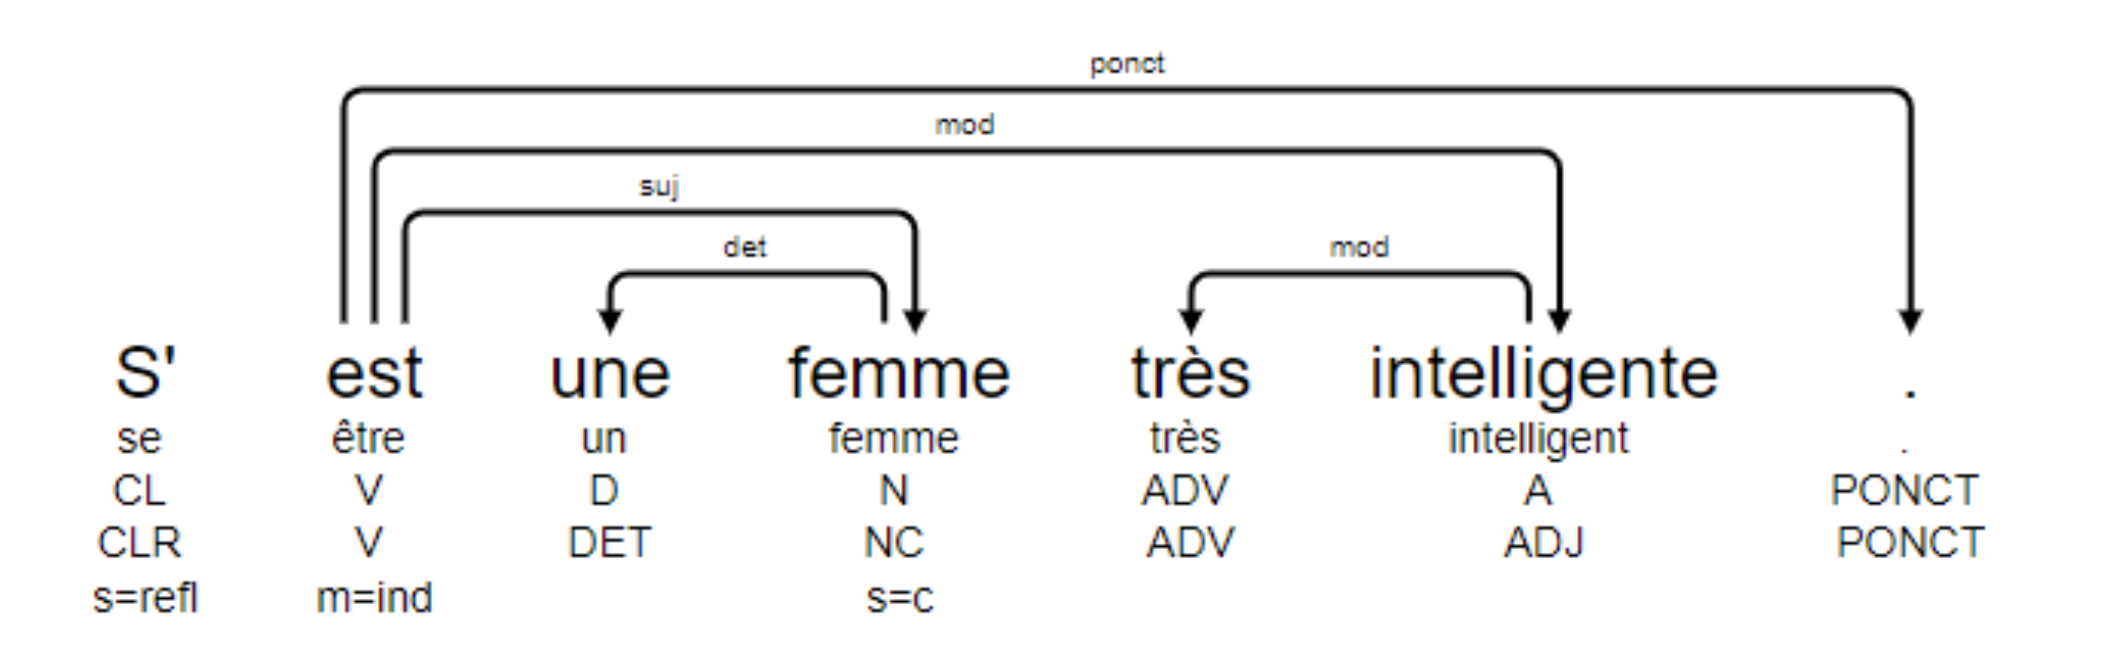
\includegraphics[width=10cm]{imgGrew.png} %l'image est retaill\'ee pour avoir une largeur de 10cm
\end{center}

Nous voyons ici que GREW n'a pas r\'{e}ussi \`{a} lier le 'S' avec les autres mots. Nous dirons par la suite qu'un graphe dans lequel un ou plusieurs mots ne sont li\'{e}s \`{a} aucun autre est un graphe qui repr\'{e}sente une qui comporte une ou plusieurs erreurs de fran\c{c}ais. Notre objectif est donc d'observer  les r\'{e}sultats de GREW sur des exemples multiples et vari\'{e}s, et d'analyser ses performances.
\newline
\newline
Tout d'abord, nous avons donc d\^{u} installer GREW, ce qui fut complexe aux vu des d\'{e}pendances de ce dernier. L'installation nous a permis d'utiliser l'outil en ligne de commande, puis par l'interm\'{e}diaire d'un script BASH, qui nous a permis d'automatiser son utilisation. L'objectif de ce script \'{e}tait de faire analyser un grand nombre de phrases par GREW, correct ou incorrect, et de v\'{e}rifier par le biais de fichier de sortie, le pourcentage de phrases bien analys\'{e}es par celui-ci. Pour se faire, nous avons regroup\'{e} les cas du fichier XML de WiCoPaCo dans un fichier CSV. Ces cas \'{e}taient repr\'{e}sent\'{e}s comme sur la photo ci-dessous :

%==== image ====
\begin{center}
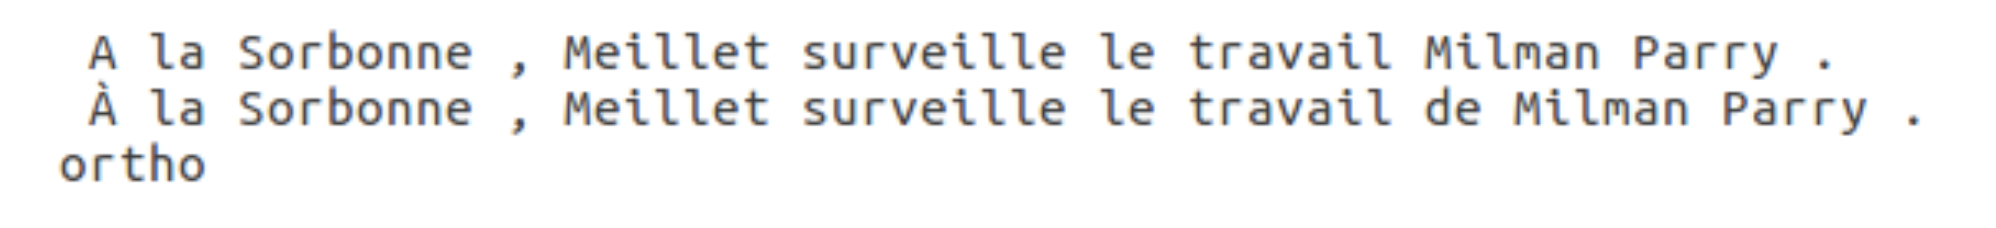
\includegraphics[width=10cm]{exemple1.png} %l'image est retaill\'ee pour avoir une largeur de 10cm
\end{center}

Chaque cas est compos\'{e} de 3 \'{e}l\'{e}ments : une phrase fausse, une phrase corrig\'{e}e, ainsi qu'un commentaire expliquant la nature de la correction. Sur cette image, la premi\`{e}re ligne correspond \`{a} la phrase avec erreur, la seconde correspond \`{a} la phrase corrig\'{e}e et la derni\`{e}re au commentaire.
\newline
\newline
De plus, une \'{e}tudiante de l'\'{e}cole T\'{e}l\'{e}com Saint-\'{e}tienne, Mme Isabelle Mornard, est venue effectuer un stage au sein du Loria, sous l'encadrement de M. Jean Lieber. Son objectif en tant que stagiaire \'{e}tait de nous aider \`{a} comprendre les diff\'{e}rentes erreurs possibles de la langue fran\c{c}aise ainsi que de les cat\'{e}goriser. En plus de cela, un de ses objectifs \'{e}tait de cr\'{e}er \`{a} la main une base de cas d'environ 200 cas regroupant des erreurs de chaque cat\'{e}gories. La base de cas a \'{e}t\'{e} remplie dans un fichier Python et chaque cas \'{e}tait repr\'{e}sent\'{e} comme ci-dessous :

%==== image ====
\begin{center}
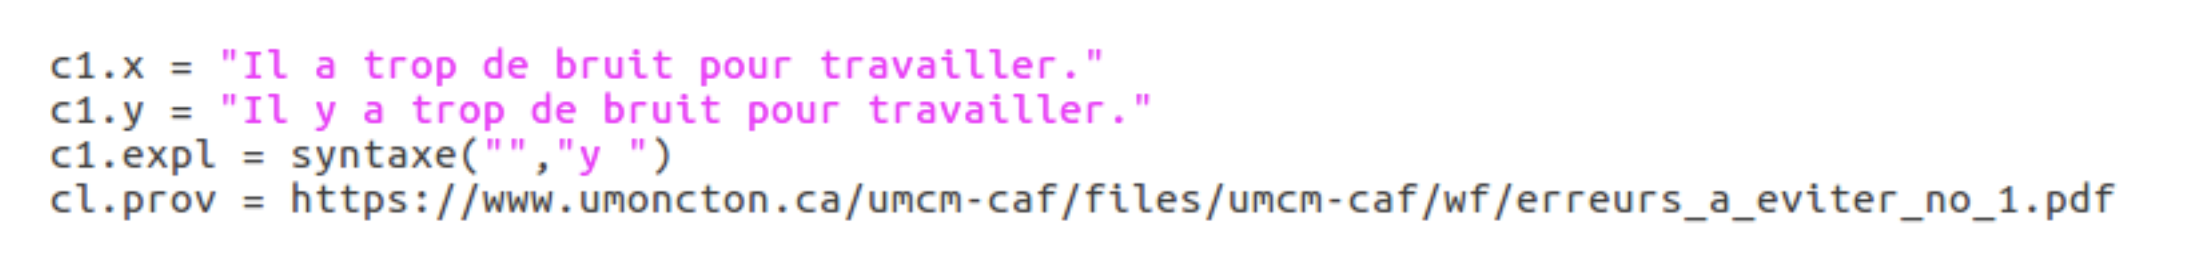
\includegraphics[width=14cm]{exemple2.png} %l'image est retaill\'ee pour avoir une largeur de 10cm
\end{center}

Un cas dans ce fichier est repr\'{e}sent\'{e} par 3 ou 4 lignes : la premi\`{e}re est une phrase avec une erreur, la seconde est une phrase correcte, la troisi\`{e}me est l'explication de la correction et la derni\`{e}re ligne est la provenance de l'exemple. La provenance est souvent est un site web de correction de fran\c{c}ais. Nous avons donc utilis\'{e} notre script sur la base de cas d'Isabelle ainsi que sur notre base de cas pour tester l'outil GREW. Les fichiers r\'{e}sultants de ces tests nous ont permis de mieux comprendre son fonctionnement ainsi que ses limites.

%==== image ====
\begin{center}
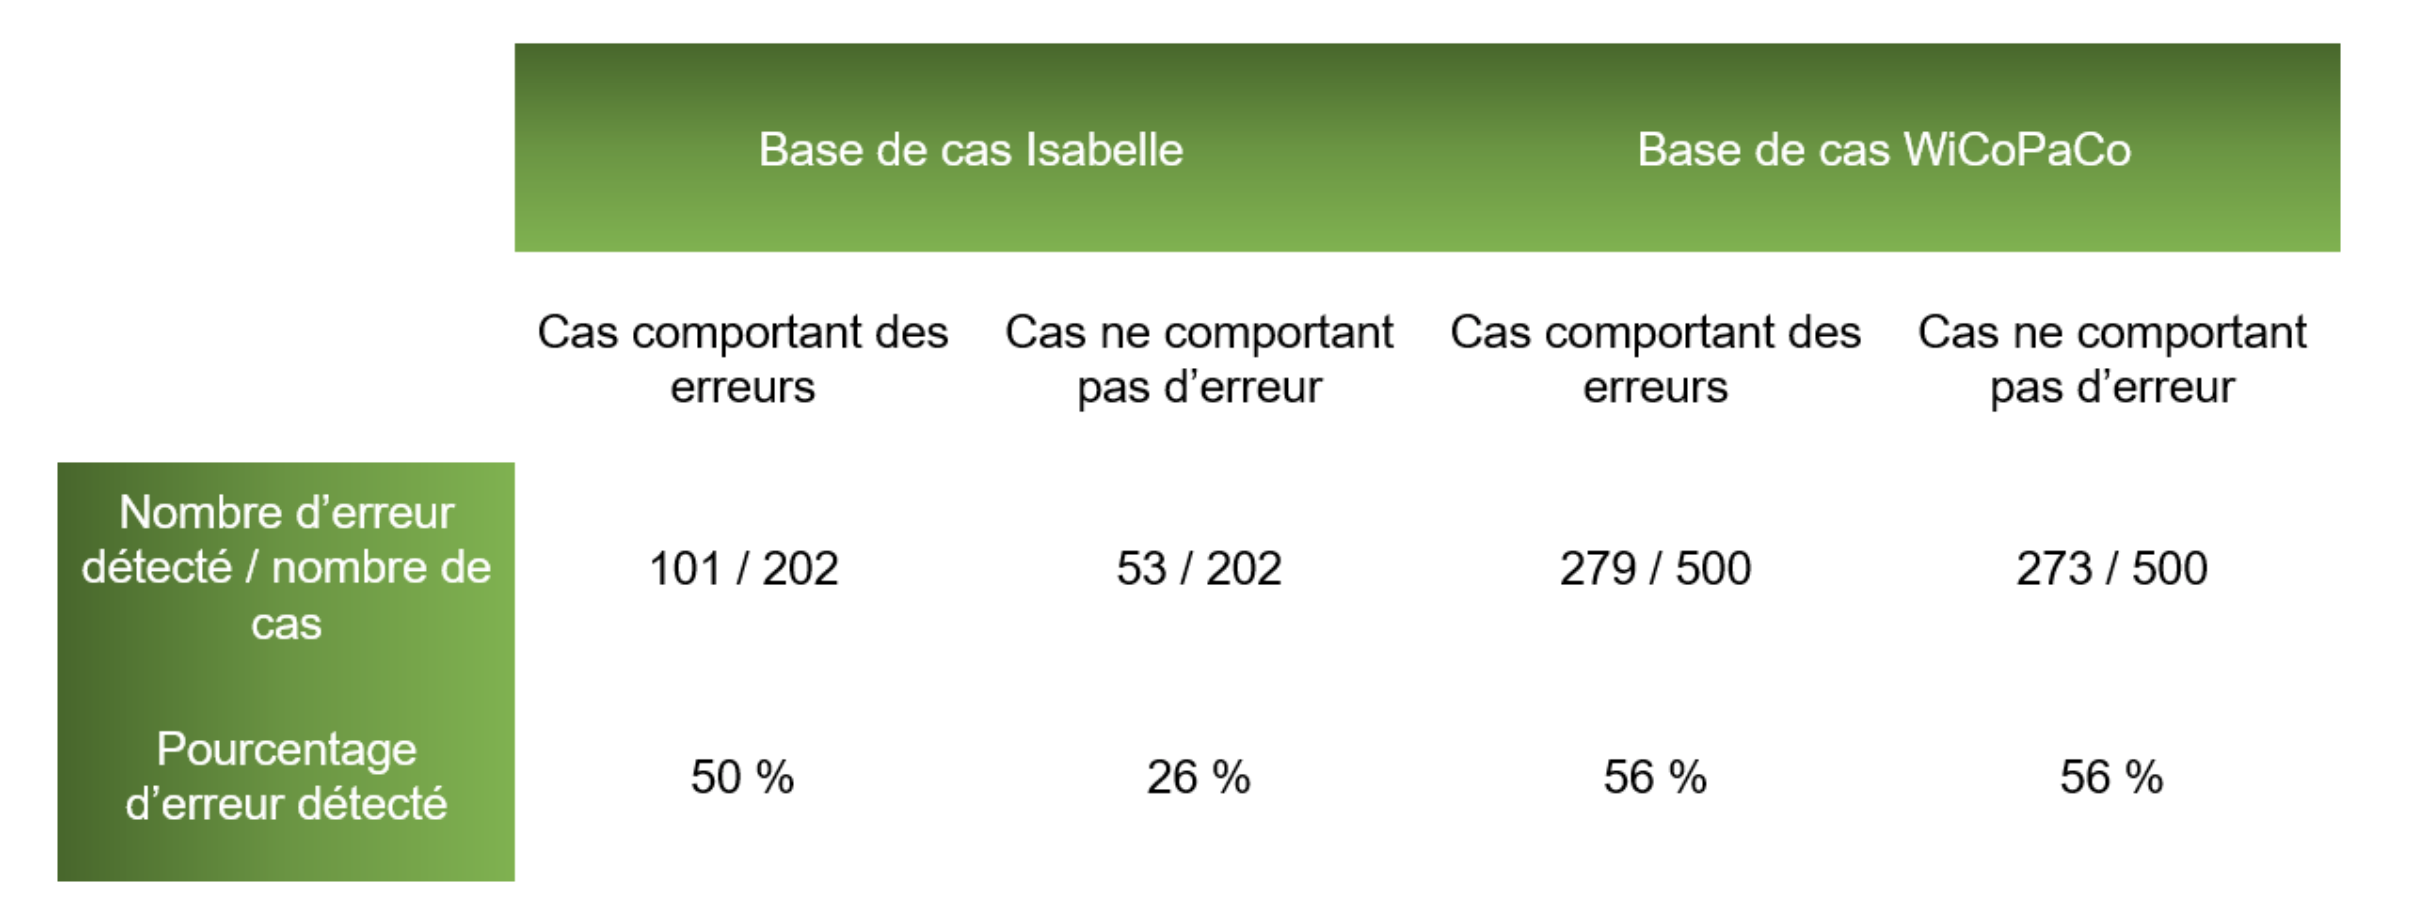
\includegraphics[width=14cm]{exemple3.png} %l'image est retaill\'ee pour avoir une largeur de 10cm
\end{center}

Les r\'{e}sultats que nous analysons dans les fichiers de sorties nous montrent que dans les cas contenant une erreur, le logiciel GREW d\'{e}tecte cette erreur une fois sur deux. Cependant, ces r\'{e}sultats nous montrent aussi que le logiciel d\'{e}tecte une erreur 40 \% du temps sur des cas ne comportant pas d'erreur. N\'{e}anmoins, nous avons r\'{e}ussi \`{a} trouver des sch\'{e}mas de phrase qui se r\'{e}p\`{e}te et pour lesquelles le logiciel ne marche pas correctement. Par exemple, tous les cas comportant des caract\`{e}res sp\'{e}ciaux tel que des accolades, des parenth\`{e}ses, des tirets, des point-virgule, des points d'interrogation, etc. sont des cas dont GREW n'arrive pas \`{a} cr\'{e}er un graphe complet correspondant et donc est consid\'{e}r\'{e} comme un cas contenant une faute m\^{e}me si ce n'est pas toujours le cas. A contrario, les cas contenant des erreurs de conjugaisons sont des cas ou un graphe complet est parfois cr\'{e}er et donc consid\'{e}r\'{e} comme sans faute. Nous pouvons donc en conclure que le logiciel GREW n'est pas infaillible quant \`{a} la d\'{e}tection d'erreur mais que des am\'{e}liorations peuvent \^{e}tre effectu\'{e} sur les cas pour pouvoir obtenir de meilleurs r\'{e}sultats.


%===== 2eme sous sous partie ====
\subsubsection{Le logiciel Java}
Notre second axe \'{e}tait la mise au point d'un outil simple permettant de traiter les donn\'{e}es des fichiers WiCoPaCo. Ces derniers se pr\'{e}sentant sous la forme suivante:
%==== image ====
\begin{center}
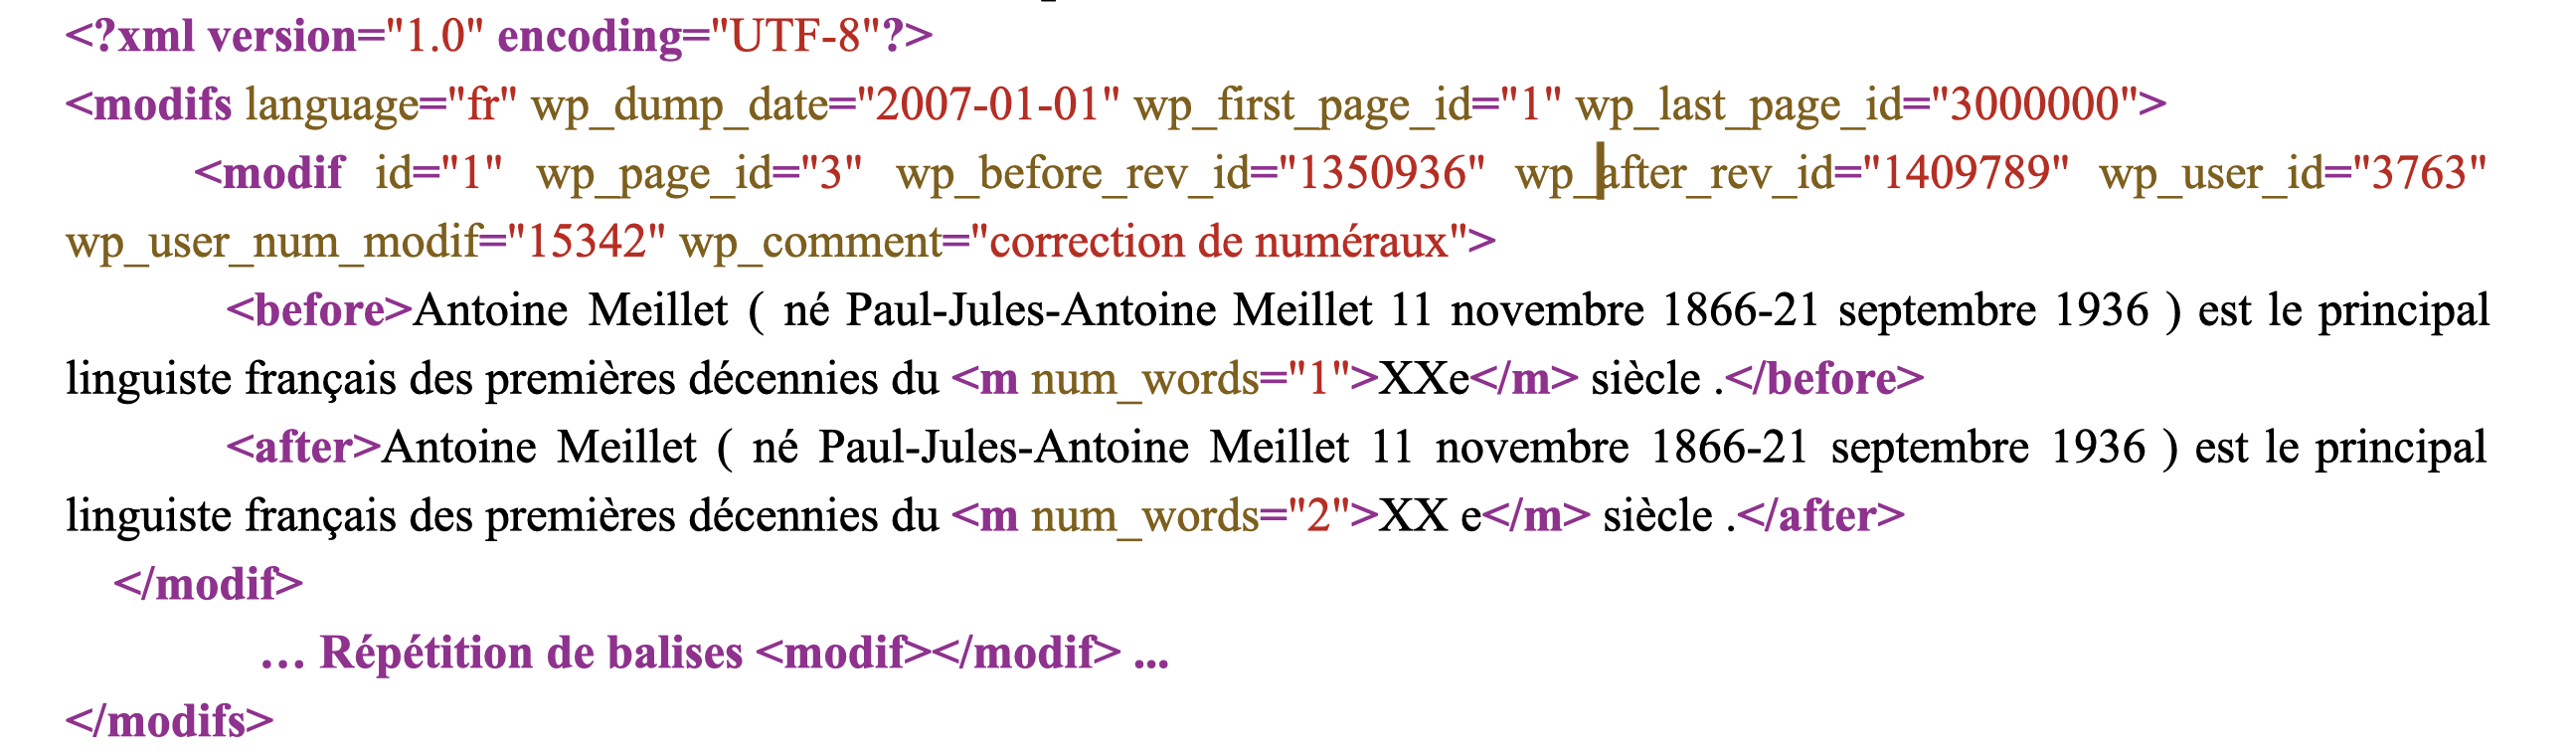
\includegraphics[width=14cm]{exemple4.png} %l'image est retaill\'ee pour avoir une largeur de 10cm
\end{center}

Les balises:
%==== image ====
\begin{center}

\includegraphics[width=7cm]{exemple5.png} %l'image est retaill\'ee pour avoir une largeur de 10cm
\end{center}

ainsi que 

%==== image ====
\begin{center}
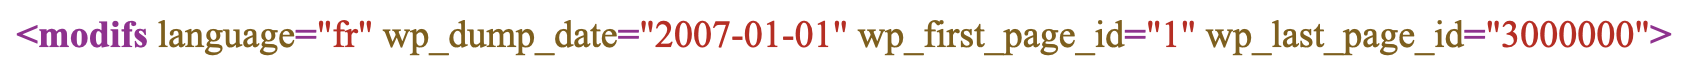
\includegraphics[width=14cm]{exemple6.png} %l'image est retaill\'ee pour avoir une largeur de 10cm
\end{center}

donnent des informations g\'{e}n\'{e}rales sur le document qui ne sont pas essentielles pour le traitement que nous d\'{e}sirons effectuer. 
Puis, suit la balise:
%==== image ====
\begin{center}
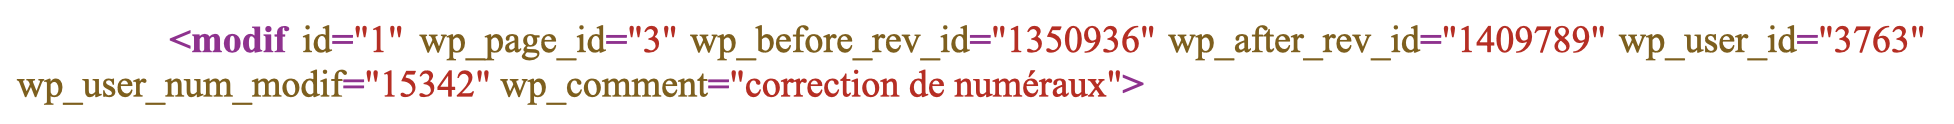
\includegraphics[width=14cm]{exemple7.png} %l'image est retaill\'ee pour avoir une largeur de 10cm
\end{center}

qui contient le contenu qui nous int\'{e}resse puisque c'est elle qui contient le cas. le document se construit de la mani\`{e}re suivante:
%==== image ====
\begin{center}
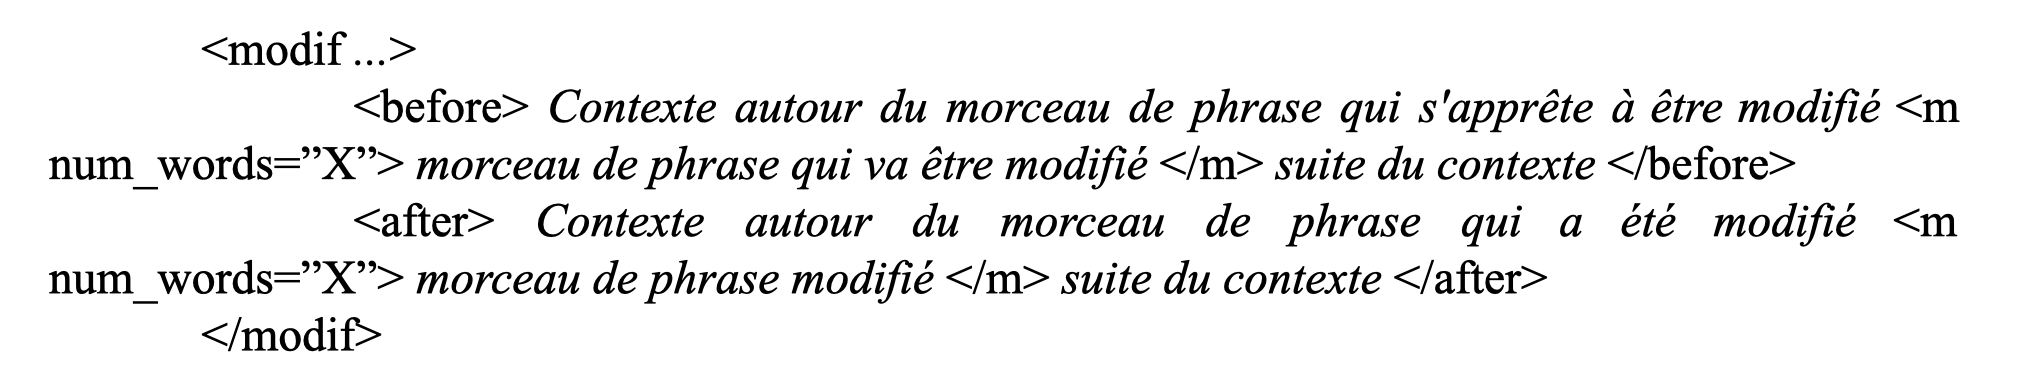
\includegraphics[width=14cm]{exemple8.png} %l'image est retaill\'ee pour avoir une largeur de 10cm
\end{center}

Donc chacune de ces balises pouvaient potentiellement correspondre \`{a} un cas qui aurait pu s'ajouter \`{a} notre base de donn\'{e}es. Or, apr\`{e}s une \'{e}tude de ces fichiers nous avons observ\'{e} que chaque balise <modif> n'\'{e}tait pas forc\'{e}ment une correction de langue, c'est pourquoi il \'{e}tait n\'{e}cessaire d'effectuer un traitement sur les donn\'{e}es.
\newline
\newline
Donc nous avons entrepris la conception d'un logiciel qui prend en entr\'{e}e un fichier au format XML tir\'{e} du site WiCoPaCo, en extrait les cas puis les traitent de sorte \`{a} enlever ceux qui ne constituent pas un cas int\'{e}ressant pour la cr\'{e}ation d'une base de cas. Enfin, il retourne les cas retenus dans un fichier au format facilement exploitable.
\newline
\newline
Ce logiciel allait contenir plusieurs filtres pouvant \^{e}tre r\'{e}partis dans des cat\'{e}gories bien pr\'{e}cises, donc nous nous sommes tourn\'{e}s vers un langage orient\'{e} objet poss\'{e}dant des propri\'{e}t\'{e}s telles que l'h\'{e}ritage. Le langage Java semblait donc bien correspondre \`{a} nos besoins gr\^{a}ce \`{a} son polymorphisme de variable, de plus il est possible de trouver en ligne de nombreuses API pour l'exploitation de fichier XML.
\newline
\newline


Apr\`{e}s r\'{e}flexion, nous avons donc d\'{e}cid\'{e} de mettre en place 3 cat\'{e}gories distinctes de filtres tel que d\'{e}crit ci-dessous:
\begin{itemize}
\item Le "globalRejector" qui accepte ou rejette un cas en fonction de l'ensemble du fichier, c'est \`{a} dire en fonction des autres cas de ce m\^{e}me fichier.
\item Le "localRejector" qui accepte ou rejette un cas en ne regardant que le cas lui m\^{e}me.
\item Le "Purifier" qui va r\'{e}duire la taille du cas en supprimant le surplus de caract\`{e}res non essentiels.
\end{itemize}
Ces 3 types de filtres s'appliquent de mani\`{e}re cons\'{e}cutive par cat\'{e}gorie sur chaque cas extrait des fichiers WiCoPaCo. Une fois l'\'{e}puration effectu\'{e}e, le logiciel cr\'{e}e un fichier de sortie contenant les cas n'ayant pas \'{e}t\'{e} rejet\'{e}s. Concernant les donn\'{e}es de sorties du logiciel, nous avons d\'{e}cid\'{e} d'utiliser le format CSV afin de pouvoir facilement ins\'{e}rer son contenu dans une base de donn\'{e}es par la suite si besoin.

%===== 2eme sous partie ====
\subsection{R\'{e}flexions sur les fonctionnalit\'{e}s}
Dans cette partie nous aborderons nos principales r\'{e}flexions qui ont orient\'{e} le d\'{e}veloppement du logiciel Java.
%===== 1ere sous sous partie ====
\subsubsection{API pour la lecture de fichier}
Comme les fichiers de WiCoPaCo sont au format XML, nous avons cherch\'{e} des API permettant une exploitation ais\'{e}e et pratique du contenu qu'il renferme. Nous avons donc utilis\'{e} l'API "DocumentBuilderFactory" ainsi que "ParserConfigurationException" provenant du package "javax.xml.parsers". Cette API permet de faire une repr\'{e}sentation en m\'{e}moire du fichier XML en un objet en structure d'arbre. Chaque noeud de cet arbre est une balise, et les enfants de ce noeud correspondent aux balises que ce noeud contient (cf illustration suivante). 

%==== image ====
\begin{center}
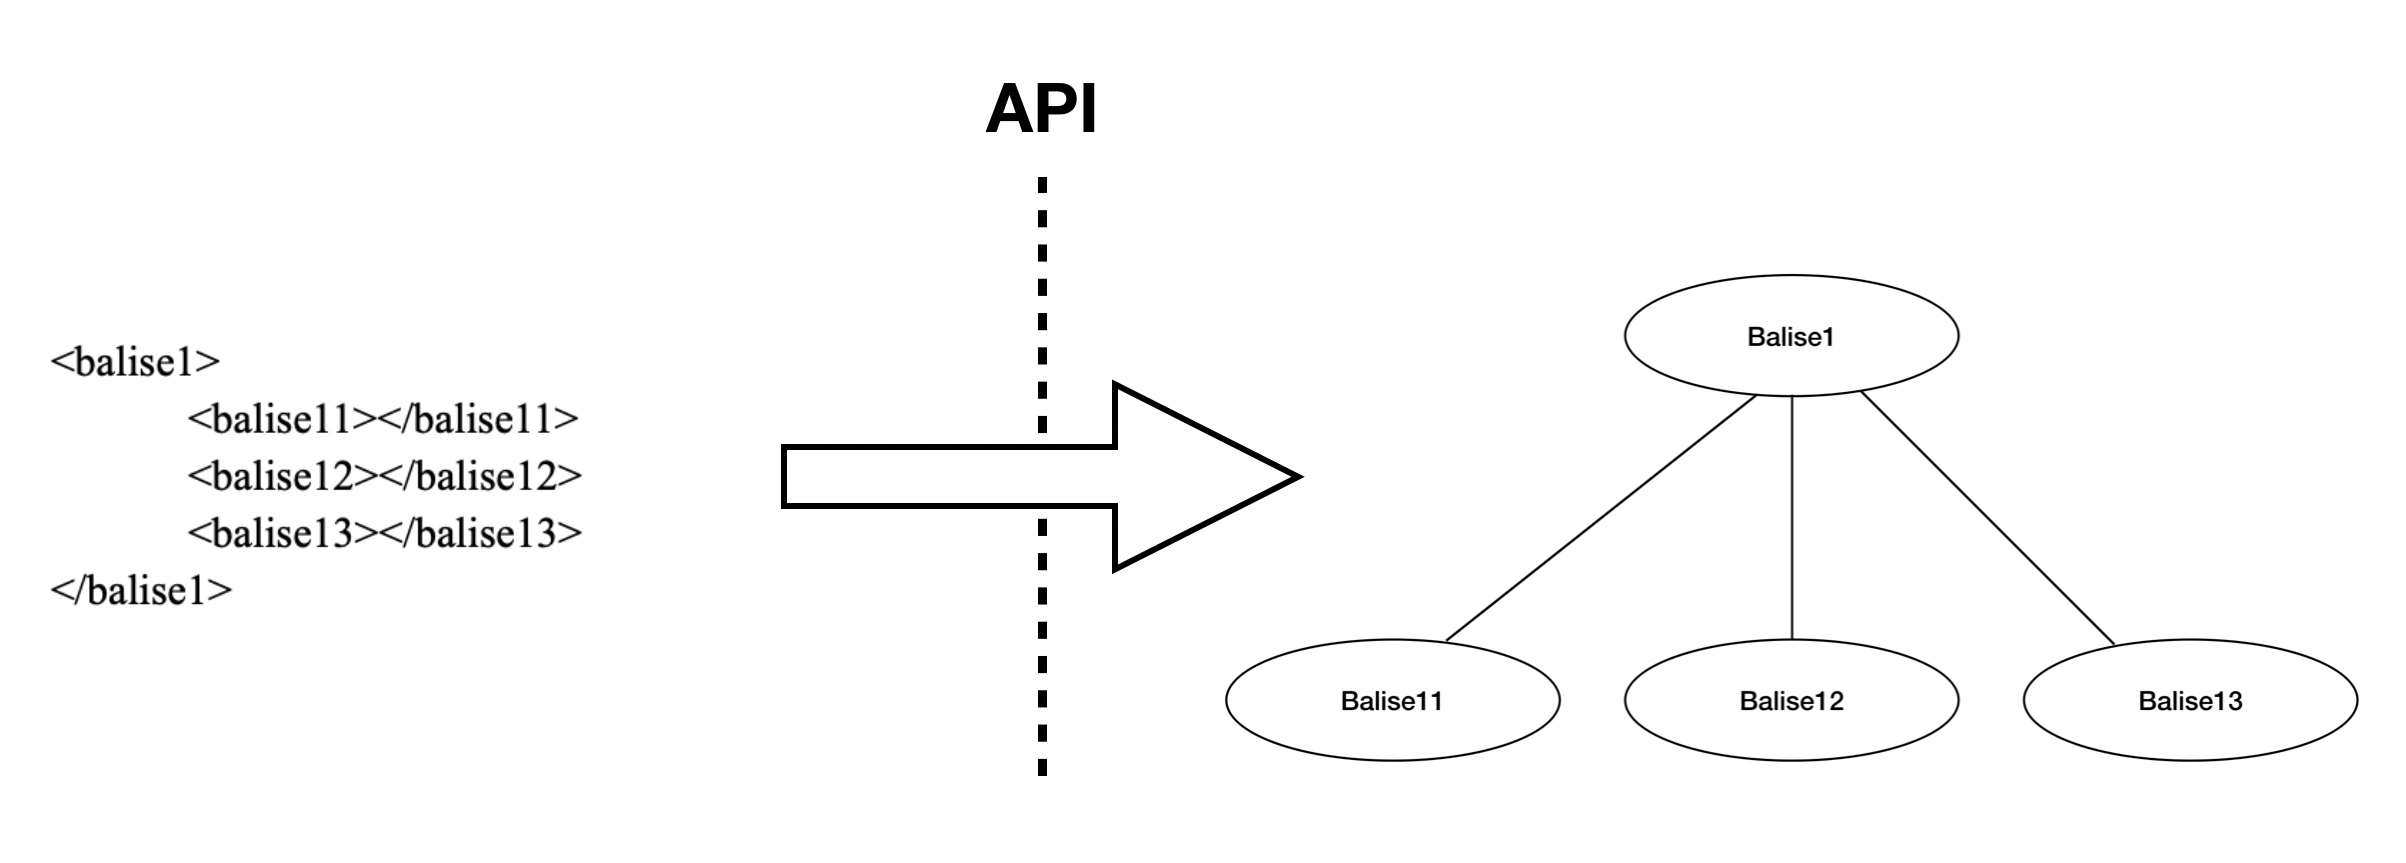
\includegraphics[width=14cm]{exemple9.png} %l'image est retaill\'ee pour avoir une largeur de 10cm
\end{center}
L'utilisation de DOM sous forme d'arbre nous permet donc une facilit\'{e} de d\'{e}veloppement pour le parcours et exploitation des balises ainsi que leurs contenus.

%===== 2eme sous sous partie ====
\subsubsection{Protocole d'ajout de filtres}
C'est ici que nous allons traiter le coeur du sujet : la mani\`{e}re dont les filtres ont \'{e}t\'{e} con\c{c}u. Ces filtres \'{e}tant un point crucial dans l'obtention d'un r\'{e}sultat int\'{e}ressant pour notre recherche, il semblait plus que n\'{e}cessaire de mettre en place un protocol rigoureux pour la validation des filtres. Le protocole \'{e}tait assez simple, mais n'en demeurait pas moins efficace.
Pour commencer, nous examinions le contenu du fichier WiCoPaCo dans le but de trouver plusieurs cas qui ne correspondaient pas \`{a} nos crit\`{e}res de s\'{e}lection. Une fois le cas relev\'{e}, il fallait l'analyser et comprendre pourquoi il ne concordait pas avec nos attentes, de sorte \`{a} trouver une r\`{e}gle nous permettant de d\'{e}tecter ce type de cas. Apr\`{e}s quoi, nous nous penchions sur la mani\`{e}re dont le filtre allait \^{e}tre impl\'{e}ment\'{e} en s'appuyant sur la r\`{e}gle que nous avions \'{e}labor\'{e}e.
Ensuite, une fois le filtre d\'{e}velopp\'{e}, une multitude de tests devaient \^{e}tre effectu\'{e}s afin de s'assurer que celui ci \'{e}tait bien fonctionnel. Nous ex\'{e}cutions donc le filtre sur un extrait du fichier de WiCoPaCo contenant quelques centaines de cas, et nous observions ceux rejet\'{e}s. Si le filtre se comportait comme nous l'attendions sur cette base test de taille r\'{e}duite, nous consid\'{e}rions que le filtre \'{e}tait fonctionnel. Si le r\'{e}sultat se r\'{e}v\'{e}lait \^{e}tre imparfait, nous entreprenions un ajustement de la r\`{e}gle jusqu'\`{a} obtention du r\'{e}sultat escompt\'{e}. 
Puis, une fois le filtre op\'{e}rationnel, une analyse statistique de l'ex\'{e}cution de ce filtre, appliqu\'{e} avec les autres filtres d\'{e}j\`{a} existant, sur le fichier entier \'{e}tait effectu\'{e}e. Le but de la d\'{e}marche \'{e}tait de d\'{e}montrer l'utilit\'{e} de ce dernier malgr\'{e} l'existence d'autres filtres. Si les r\'{e}sultats statistiques attestaient de l'int\'{e}r\^{e}t du filtre, alors ce dernier \'{e}tait accept\'{e} et ajout\'{e} au projet.
Enfin, nous appliquions tous les filtres sur les quelques 400 000 cas et entreprenions une nouvelle analyse sur le fichier de sortie du logiciel en qu\^{e}te de cas ne correspondant pas \`{a} nos crit\`{e}res pour recommencer le protocole.

%===== 3eme sous sous partie ====
\subsubsection{Fichier de sortie}
Le logiciel, une fois les filtres appliqu\'{e}s sur un fichier pass\'{e} en entr\'{e}, devait produire une sortie exploitable facilement. C'est pourquoi nous avons d\'{e}cid\'{e} d'utiliser le format CSV. C'est un format simple, exportable, lisible par un humaine sous forme de tableau, et qui peut \^{e}tre ais\'{e}ment ins\'{e}rer dans une base de donn\'{e}es via un script si besoin en est. Chaque ligne correspond \`{a} un cas, et le fichier se forme en trois colonnes : la premi\`{e}re correspond au cas avant que la correction soit effectu\'{e}e, la seconde \'{e}tant le cas avec la correction, et la troisi\`{e}me colonne se trouve \^{e}tre l'\'{e}ventuel commentaire que l'auteur de la correction peut faire sur la correction qu'il effectue sur wikipedia.
Il est \'{e}galement possible d'activer la sortie pour chacun des filtres, chaque fichier de sortie porte le nom de "RejectedBy" concat\'{e}n\'{e} avec le nom du filtre et contient les cas rejet\'{e}s. Cela permet de voir ce que chaque filtre a effectu\'{e} lors de l'ex\'{e}cution.

%===== 3eme sous partie ====
\subsection{D\'{e}tail sur les diff\'{e}rents filtres}
%===== 1ere sous sous partie ====
\subsubsection{Le type GlobalRejector}
Comme expliqu\'{e} de mani\`{e}re succincte plus t\^{o}t, le type de filtre GlobalRejector est une cat\'{e}gorie contenant les filtres qui n\'{e}cessite une analyse enti\`{e}re du document d'entr\'{e}e, pour y collecter des informations, afin de statuer sur l'acceptation d'un cas. 
	Dans cette cat\'{e}gorie se trouve deux filtres:
Le premier \'{e}tant le "RollbackFilter", qui a pour but de refuser les retours sur correction. Le filtre parcourt une premi\`{e}re fois enti\`{e}rement le fichier en r\'{e}pertoriant chaque correction, puis lors du parcours du document pour le traitement des cas, le filtre scrute ses donn\'{e}es pour voir si une modification inverse est effectu\'{e}e \`{a} un moment. S'il existe une modification inverse dans le document, alors le cas est rejet\'{e}.
Voici un exemple que le RollbackFilter rejette :
On trouve une premi\`{e}re modification comme suit,
%==== image ====
\begin{center}
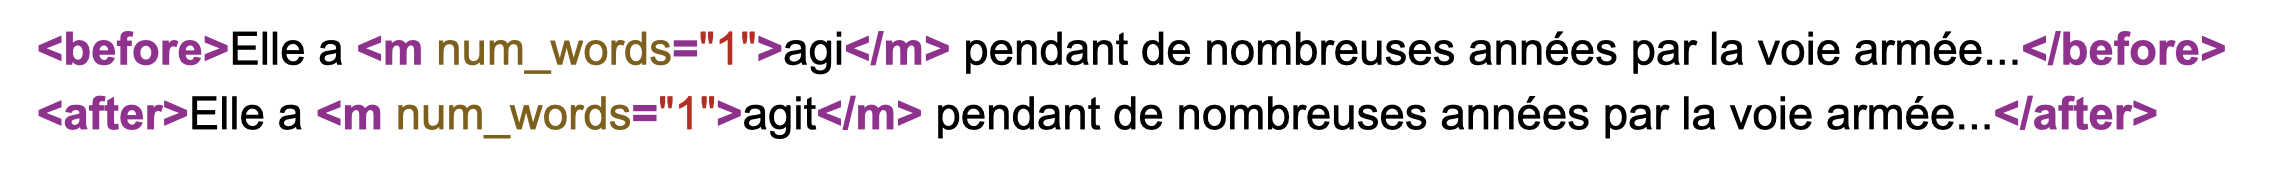
\includegraphics[width=14cm]{exemple10.png} %l'image est retaill\'ee pour avoir une largeur de 10cm
\end{center}

Puis, plus loin dans le document on trouve la correction inverse,

%==== image ====
\begin{center}
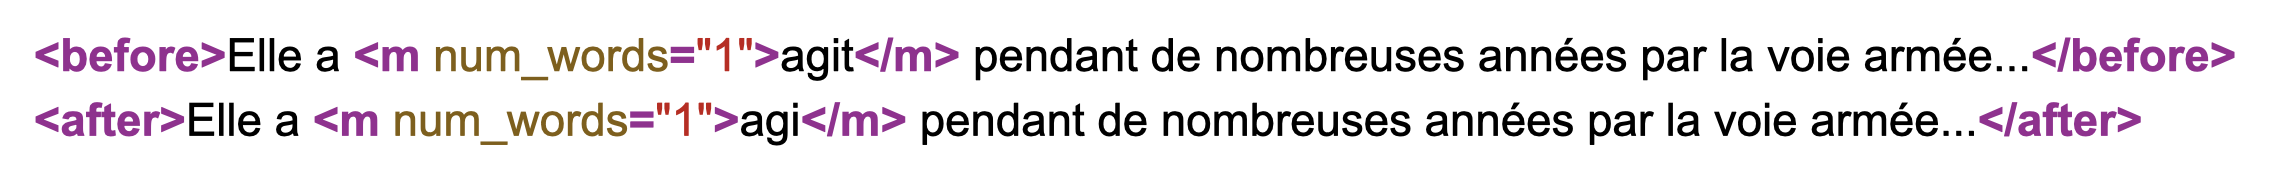
\includegraphics[width=14cm]{exemple11.png} %l'image est retaill\'ee pour avoir une largeur de 10cm
\end{center}

Le second filtre de cette cat\'{e}gorie se nomme "SpellingErrorLabel", ce dernier est diff\'{e}rents des autres filtres, car il repose sur une \'{e}tude effectu\'{e}e sur WiCoPaCo faite par des chercheurs travaillant au LIMSI. Au sein de leurs r\'{e}sultats de recherche se trouve un fichier XML contenant les identifiants des cas comportant des erreurs lexicales, ainsi que des erreurs grammaticales. Donc le filtre r\'{e}pertorie les identifiants not\'{e}s par l'\'{e}quipe de chercheurs et rejette les cas dont l'identifiant n'appartient pas \`{a} ceux qui ont \'{e}t\'{e} relev\'{e}s par l'\'{e}quipe travaillant au LIMSI.

%===== 2eme sous sous partie ====
\subsubsection{Le type LocalRejector}
Quand au type "LocalRejector", c'est une cat\'{e}gorie comprenant des filtres qui inspecte uniquement le cas et son contenu pour d\'{e}cider si le cas est rejet\'{e}. 
	Deux filtres ont \'{e}t\'{e} impl\'{e}ment\'{e} dans cette cat\'{e}gorie:
Le premier porte le nom de "EstheticalRestructurationRejector" et a pour but de d\'{e}tecter les reformulations ou restructuration de phrases. Pour ce faire, notre filtre utilise la distance d'\'{e}dition de Levenshtein. Un cas est rejet\'{e} si la partie "correction effectu\'{e}e" a un nombre de caract\`{e}res inf\'{e}rieur \`{a} 4 et que la distance de Levenshtein est plus grande que la moiti\'{e} du mot le plus court, ou si la partie correction a un nombre de caract\`{e}res sup\'{e}rieur \`{a} 4 et que la distance calcul\'{e}e est plus grande que la moiti\'{e} de la plus petites partie modification.
Voici un exemple que le EstheticalRestructurationRejector rejette :
%==== image ====
\begin{center}
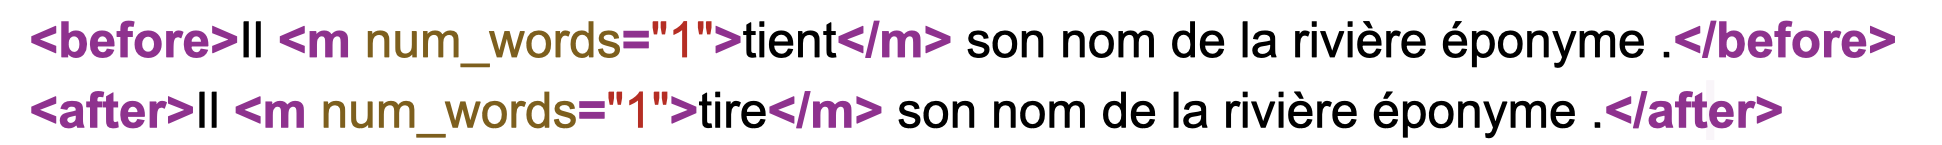
\includegraphics[width=12cm]{exemple12.png} %l'image est retaill\'ee pour avoir une largeur de 10cm
\end{center}
Le deuxi\`{e}me, "NumberRejector" \'{e}limine les corrections portant sur les chiffres, car ce sont des corrections de contenu (date, pourcentage, ...) et donc, elles ne constituent pas d'erreurs de fran\c{c}ais. 
Voici un exemple que le NumberRejector rejette :
%==== image ====
\begin{center}
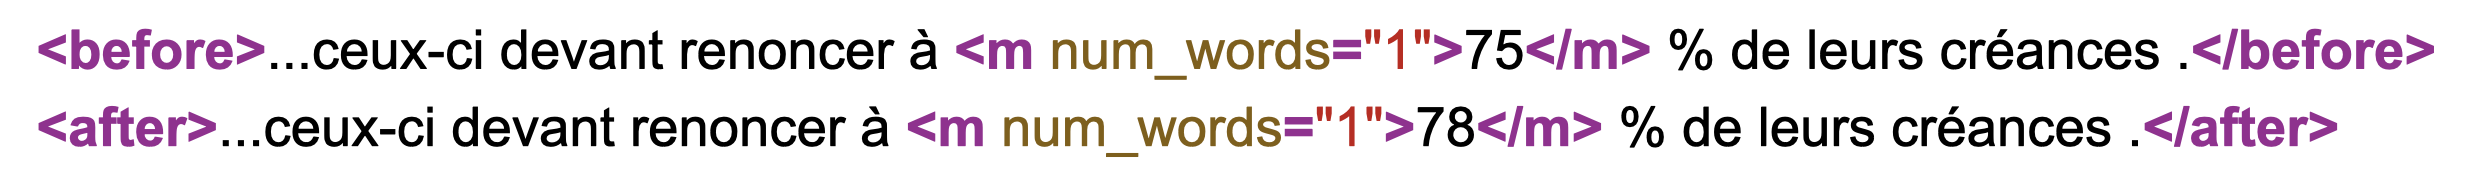
\includegraphics[width=14cm]{exemple13.png} %l'image est retaill\'ee pour avoir une largeur de 10cm
\end{center}

%===== 3eme sous sous partie ====
\subsubsection{Le type Purifier}
Enfin la derni\`{e}re cat\'{e}gorie de filtre: "PurifierFilter". Cette cat\'{e}gorie est diff\'{e}rente des pr\'{e}c\'{e}dentes car son but n'\'{e}tant pas d'accepter ou de rejeter un cas, mais d'\'{e}liminer le contenu inutile que comporte certains cas. Ce type de filtre travaille \`{a} l'\'{e}chelle du cas, et se cantonne \`{a} \'{e}liminer des caract\`{e}res.
	Cette cat\'{e}gorie contient deux filtres:
Le filtre "SentencePurifier" a pour mission de supprimer tout le contenu superflu autour de la correction, et de n'en garder que le noyau. Le probl\`{e}me \'{e}tant que les cas contenus dans le fichier de WiCoPaCo sont souvent entour\'{e}s du contexte, ce qui n'est pas important pour l'utilisation que nous voulons en faire. C'est pourquoi nous avons d\'{e}cid\'{e} de supprimer le contexte, dans l'optique d'all\'{e}ger le fichier de sortie
Par exemple le cas : 
%==== image ====
\begin{center}
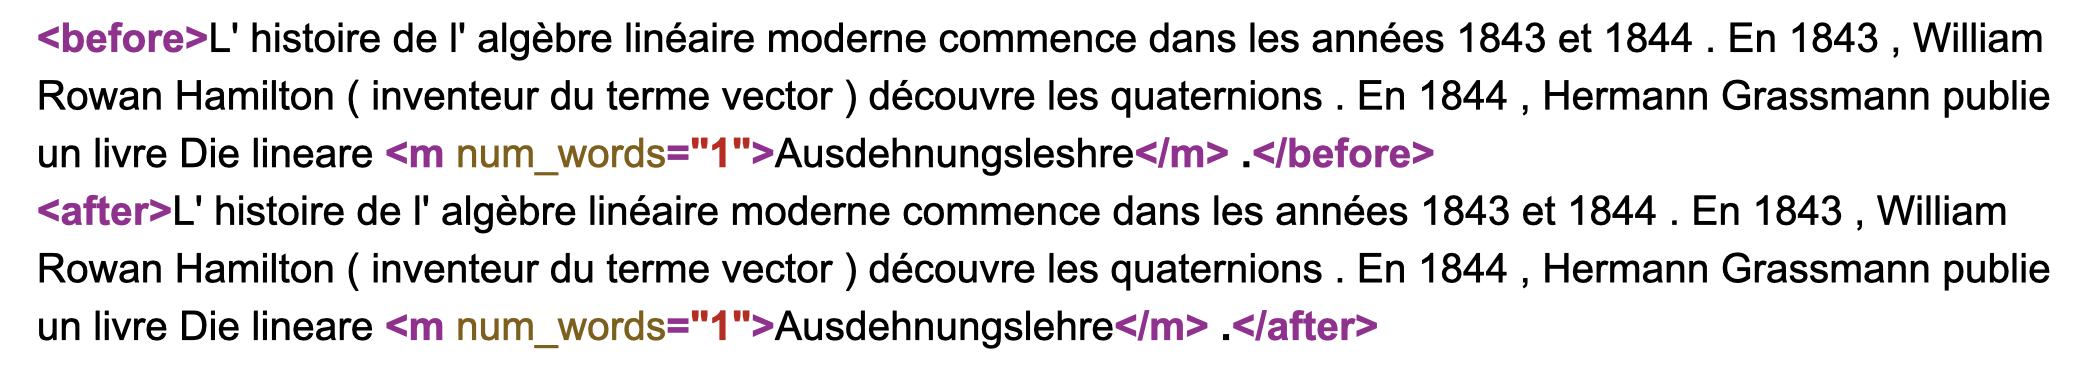
\includegraphics[width=14cm]{exemple14.png} %l'image est retaill\'ee pour avoir une largeur de 10cm
\end{center}
va se transformer par l'application du filtre SentencePurifier en : 
%==== image ====
\begin{center}
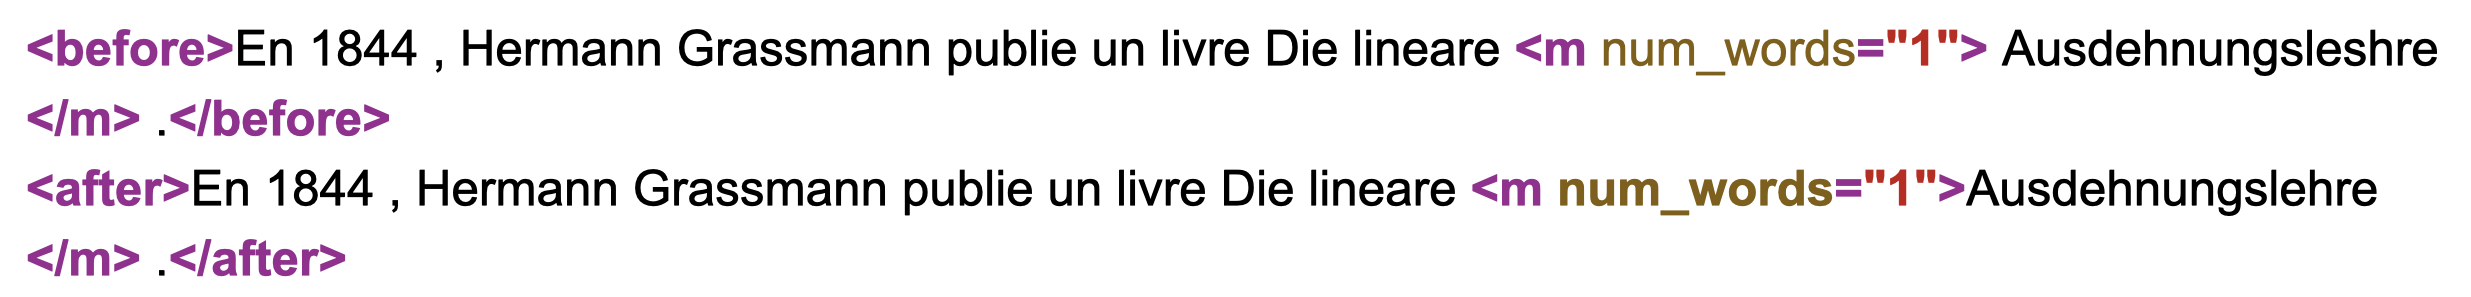
\includegraphics[width=14cm]{exemple15.png} %l'image est retaill\'ee pour avoir une largeur de 10cm
\end{center}
Enfin, le filtre SpecialCaracterPurifier, est assez simple. Il consiste \`{a} supprimer les caract\`{e}res sp\'{e}ciaux suivant: "\$", "*" , "/", "\#" , se trouvant au d\'{e}but de la premi\`{e}re phrase des cas. Les corrections pouvant \^{e}tre effectu\'{e}e sur tout le contenu de la page, certains cas sont des annotations en pied de page et ont donc une mise en forme particuli\`{e}re.
Ce filtre n'a d'int\'{e}r\^{e}t que s'il est appliqu\'{e} apr\`{e}s le filtre "SentencePurifier", car il risquerait d'effectuer le m\^{e}me travail

%===== 3ere partie ====
\section{R\'{e}sultats}

%===== 1ere sous partie ====
\subsection{Statistiques}

%===== 1ere sous sous partie ====
\subsubsection{Les filtres GlobalRejector}
contenu:
statistiques de chaque filtre 
pour chaque filtres :
\begin{itemize}
\item nombre de cas enlev\'{e} (nombre et pourcentage) sur la base de test, puis sur tout le fichier de WiCoPaCo
\item temps d'ex\'{e}cution
\end{itemize}

%===== 2eme sous sous partie ====
\subsubsection{Les filtres LocalRejector}
contenu:
de meme que la sous sous partie precedente

%===== 3eme sous sous partie ====
\subsubsection{Les filtres Purifier}
contenu:
de meme que la partie sous sous precedente

%===== 2eme sous partie ====
\subsection{R\'{e}sultat final}
contenu:
comparaison entre le fichiers WiCoPaCo de base et la pseudo base de cas obtenue:
\begin{itemize}
\item Nombre de cas enlev\'{e} au total
\item Nombre de cas \'{e}pur\'{e} au total
\item Temps de traitement des donn\'{e}es
\end{itemize}

%===== 3eme sous partie ====
\subsection{Ouverture}
contenu:
\begin{itemize}
\item Les difficult\'{e}s rencontr\'{e}s au cours de notre initiation \`{a} la recherche
\item Le travail qu'il reste \`{a} accomplir (finir l'\'{e}puration de la base de cas puis rem\'{e}moration et adaptation pour obtenir un logiciel fonctionnel)
\end{itemize}


\end{document}

